% !TEX root = ../../../under-spec-z.tex

\subsection{Schemes} % (fold)
\label{sub:schemes}

    % \vspace{-2em}
    % \begin{translation}{2.4}{1}
    %     In this section we present the main definition of this paper, that of a \emph{scheme over $\ccat$}.
    %     For this, we start by introducing the idea of an open Zariski cover in $\Shv(\aff{\ccat})$, and will define schemes as sheaves possessing an open Zariski cover of affine schemes.
    %     We will then demonstrate some fundamental properties of schemes (for example, gluing, and stability under pullbacks and disjoint unions).
    % \end{translation}

    \begin{quotation}
        \emph{In this section we present the main definition of this paper, that of a \emph{scheme over $\ccat$}.} (\S2.4,~\P1)
    \end{quotation}

    \subsubsection{Using sheaves} % (fold)
    \label{ssub:using_sheaves}

        % At the end of \cref{sub:the_zariski_topology} we showed how we can consider the category $\aff{\ccat}$ of affine schemes as being embedded inside $\Shv^{\text{fpqc}}(\aff{\ccat})$, and then slightly broaden our definition of affine schemes to include any (Zariski) sheaf in the essential image of this embedding (that is, close the collection of affine schemes under isomorphism).
        % \Cref{df:zariski-open-morphism,df:fpqc-zariski-covers} define what it means for a morphism of affine schemes \emph{as objects of $\aff{\ccat}=\op{\comm{\ccat}}$} to be Zariski open, but we should now give equivalent conditions for when a morphism of affine schemes \emph{as objects of $\ASch(\ccat)$} is Zariski open.
        % We use \cref{df:zariski-open-sheaves} as our temporary definition for this latter scenario, and then prove that it is equivalent to our previous definition in \cref{le:zariski-open-sheaves-and-morphisms}.

        In light of \cref{eq:both-types-of-affine-schemes}, we need to rephrase \cref{df:zariski-open-morphism,df:fpqc-zariski-covers} in terms of sheaves.

        \begin{definition}[Zariski open in {$\Shv(\aff{\ccat})$} {(Définition~2.12,~\S2.4,~p.18)}]\label{df:zariski-open-sheaves}
            \mbox{}\vspace{-1em}
            \begin{enumerate}[(i)]
                \item Let $X\in\ASch(\ccat)$ and $F\subset X$ a subsheaf of $X$.
                    We say that $F$ is \emph{Zariski open in $X$} if there exists a Zariski-open (in the sense of \cref{df:zariski-open-morphism}\footnote{
                        Recall \cref{df:affine-schemes-general}: $X$ is not necessarily in $\aff{\ccat}$, but we know that we can find some $\spec B\in\aff{\ccat}$ such that $X\cong\Hom(\blank,\spec B)$.
                        Similarly we can find $\spec B_i\in\aff{\ccat}$ such that $X_i\cong\Hom(\blank,\spec B_i)$.
                        Then we want the family $\{\spec B_i\to\spec B\}_{i\in I}$ to be Zariski open in the sense of \cref{df:zariski-open-morphism}.
                    }) family $\{X_i\to X\}_{i\in I}$ in $\aff{\ccat}$ (where $I$ is \emph{not} necessarily finite\footnote{
                        See the paragraph accompanying \cref{fg:infinitely-many-lines,fg:disjointlines}, just before \cref{ssub:partial_summary}.
                    }) and a sheaf morphism $\coprod_{i\in I}X_i\to X$ whose image in $X$ is $F$.
                \item A morphism $f\colon F\to G$ in $\Shv(\aff{\ccat})$ is \emph{Zariski open} (or an \emph{open Zariski immersion}) if, for all affine schemes $X$ and morphisms $X\to G$, the induced morphism
                \begin{equation*}
                    F\times_G X\to X
                \end{equation*}
                is a monomorphism whose image is Zariski open in $X$.\qedhere
            \end{enumerate}
        \end{definition}

        By definition, Zariski-open morphisms are stable under a change of base and also under composition in $\Shv(\aff{\ccat})$.
        Further, \emph{it can be easily checked that Zariski-open morphisms are monomorphisms in $\Shv(\aff{\ccat})$.} (\S2.4,~\P2)
        When we introduce schemes we will see that this point about monomorphisms is an example of a property holding on all affine schemes in a cover implying that the same property holds for the whole scheme, i.e. `locally a monomorphism implies globally a monomorphism'.

        \bigskip

        At the moment we have two definitions for what it means for a morphism of affine schemes to be Zariski open: \cref{df:zariski-open-morphism} for $\aff{\ccat}$; and \cref{df:zariski-open-sheaves} for $\ASch(\ccat)$.
        The following lemma shows that the two definitions are indeed equivalent.

        \begin{lemma}[\mbox{}{Lemme~2.14,~\S2.4,~p.18}]\label{le:zariski-open-sheaves-and-morphisms}
            Let $f\colon Z\to Y$ be a morphism of affine schemes.
            Then $f$ is Zariski open in the sense of \cref{df:zariski-open-morphism} if and only if it is Zariski open in the sense of \cref{df:zariski-open-sheaves}.
        \end{lemma}

        \begin{proof}
            This proof is largely unpacking definitions, and is given in \cite{Toen:2005wxa}.
        \end{proof}

        \begin{definition}[Scheme relative to $\ccat$ {(Définition~2.15,~\S2.4,~p.19)}]\label{df:relative-scheme}
            A sheaf $F\in\Shv(\aff{\ccat})$ is a \emph{scheme relative to $\ccat$} (or simply a \emph{scheme} if the context is clear) if there exists a family $\{X_i\}_{i\in I}$ of affine schemes and a morphism
            \begin{equation*}
                p\colon\left(\coprod_{i\in I}X_i\right)\to F
            \end{equation*}
            satisfying the following two conditions:
            \begin{enumerate}[(i)]
                \item $p$ is an epimorphism of sheaves;
                \item for all $i\in I$ the morphism\footnote{
                    That is, the induced morphism $X_i\to\coprod X_i\to F$.
                } $X_i\to F$ is an open Zariski immersion.
            \end{enumerate}
            We define the category $\Sch(\ccat)$ to be the full subcategory of $\Shv(\aff{\ccat})$ consisting of such sheaves, and call the family $\{X_i\to X\}$ an \mbox{\emph{affine Zariski cover of $F$}}.
        \end{definition}

        At the moment, we simply know that a scheme is in some sense `covered' by affine schemes -- we do not yet know exactly how these affine schemes `fit together' (we find out in \cref{le:actual-gluing}).
    
        \begin{figure}[h]
            \centering
            \frame{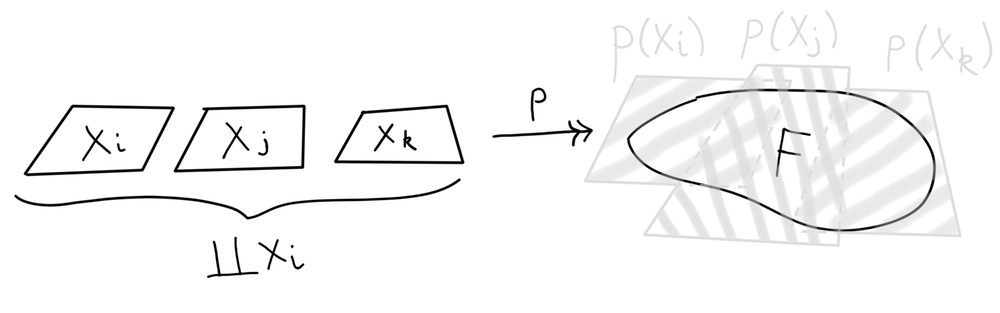
\includegraphics[width=\textwidth]{images/scheme.png}}
            \caption{\Cref{df:relative-scheme} -- schemes}
            \label{fg:scheme}
        \end{figure}

        When we defined Zariski covers in \cref{df:fpqc-zariski-covers} we required them to be finitely conservative, but here we don't have any finiteness conditions -- we use the word `cover' in two slightly different senses.
        Here it is not so much a topological cover, as a scheme-theoretic cover.
        Locally, schemes `look like' affine schemes, which have this finitely conservative (i.e. \emph{quasi-compact}) property, but globally they are not under such tight restrictions.
        See \cref{fg:infinitely-many-lines,fg:disjointlines}.

        \begin{figure}[h]
            \begin{minipage}{0.48\textwidth}
                \centering
                \frame{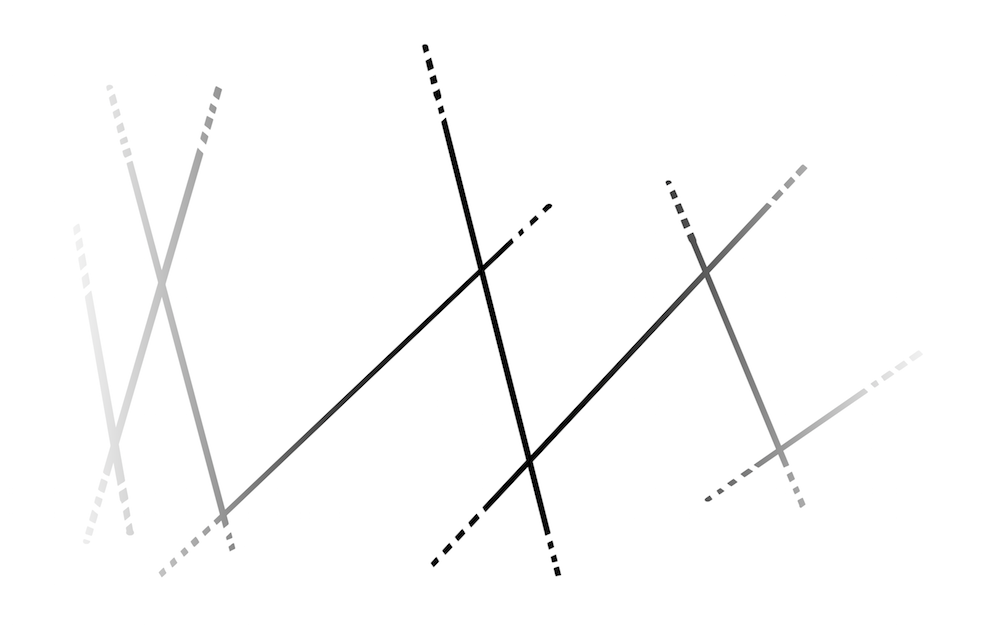
\includegraphics[width=\textwidth]{images/infinitely-many-lines.png}}
                \caption{Consider infinitely many lines glued together pairwise at a point -- this is a scheme, since we can take the $X_i$ to be the lines, then $\{X_i\}$ is an \emph{infinite} affine Zariski cover}
                \label{fg:infinitely-many-lines}
            \end{minipage}
            \hfill
            \begin{minipage}{0.45\textwidth}
                \centering
                \frame{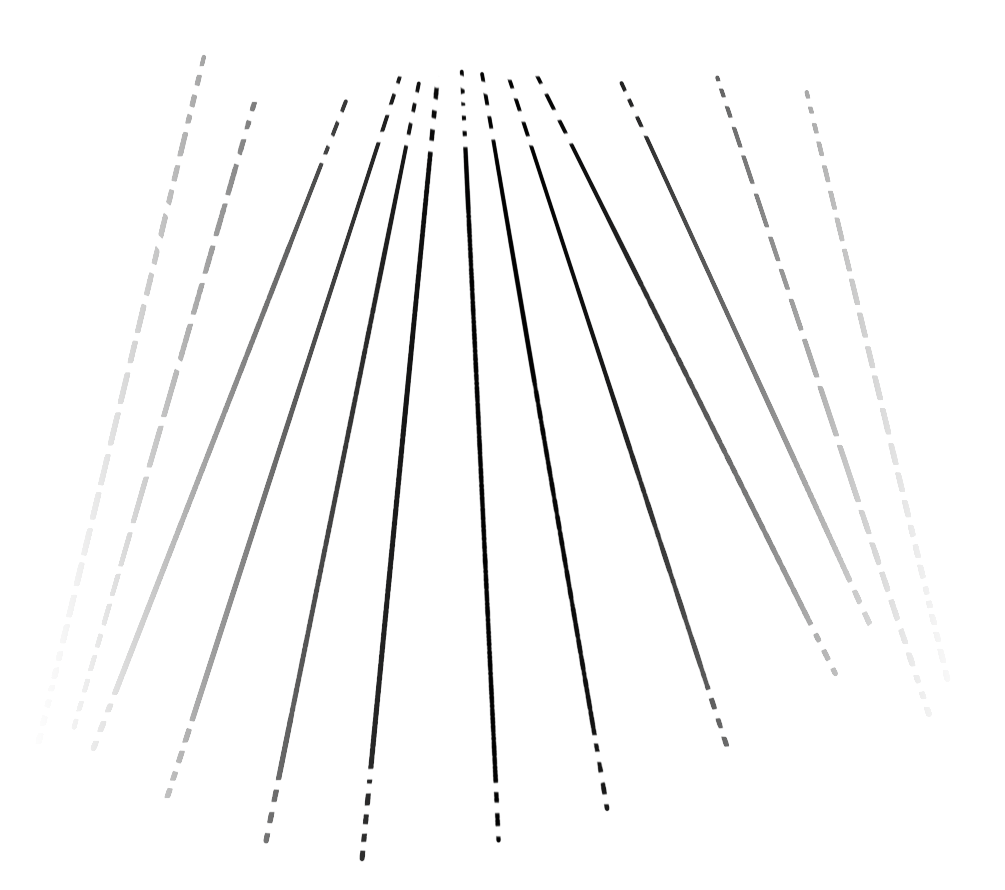
\includegraphics[width=\textwidth]{images/disjointlines.png}}
                \caption{The trivial gluing (coproduct) of infinitely many lines; here we can take the $X_i$ to be the lines and $p$ to simply be the identity}
                \label{fg:disjointlines}
            \end{minipage}
        \end{figure}

    % subsubsection using_sheaves (end)




    \subsubsection{Partial summary} % (fold)
    \label{ssub:partial_summary}

        Before moving on to talk about the properties schemes, we provide a brief summary of what we have done so far.

        In \cref{ssub:zariski_covers} we defined two topologies on $\aff{\ccat}=\op{\comm{\ccat}}$ by defining certain types of \emph{open} morphisms: \emph{fpqc} and \emph{Zariski}.
        After this, in \cref{ssub:sheaves}, we looked at a more abstract situation: using the topologies we just defined to consider fpqc and Zariski \emph{sheaves}\footnote{
            Then agreeing, from now on, to say \emph{sheaf} to mean a \emph{Zariski} sheaf.
        }.
        Then, with the Yoneda embedding, we considered $\aff{\ccat}$ as sitting inside $\Shv^\text{fpqc}(\aff{\ccat})\subset\PShv(\aff{\ccat})$, and called the essential image of this embedding $\ASch(\ccat)$, whose objects are \emph{affine schemes}.
        % \begin{equation}\label{eq:diagram-of-inclusions}
        %     \begin{array}{ccccccccc}
        %         & & &\tightoverset{close under isomorphism}{\big\downarrow} & & & &\tightoverset{ignore topology (coarser)}{\big\downarrow} &\\
        %         \aff{\ccat} &\hookrightarrow &\Shv^{\text{fpqc}}(\aff{\ccat}) &\subset &\ASch(\ccat) &\subset &\Shv(\aff{\ccat}) &\subset &\PShv(\aff{\ccat})\\
        %         &\tightunderset{Yoneda functor}{\big\uparrow} & & & &\tightunderset{pass to Zariski topology}{\big\uparrow} & & &
        %     \end{array}
        % \end{equation}
        Next, in \cref{df:zariski-open-sheaves}, we extended our definition of Zariski open morphisms to general sheaf morphisms and showed that it agreed with our previous definition.
        We used this to define a \emph{scheme} as a sheaf that was covered by affine schemes, with each affine scheme embedding into the sheaf via a Zariski open immersion.
        By definition, every affine scheme is also a scheme (just as we would expect) and every scheme is a sheaf.
        \Cref{fg:hierarchy} shows how all these full subcategories overlap inside $\PShv(\aff{\ccat})$.
    
        \begin{figure}[h!]
            \centering
            \begin{minipage}[t]{0.65\textwidth}
                \vspace{0pt}
                \frame{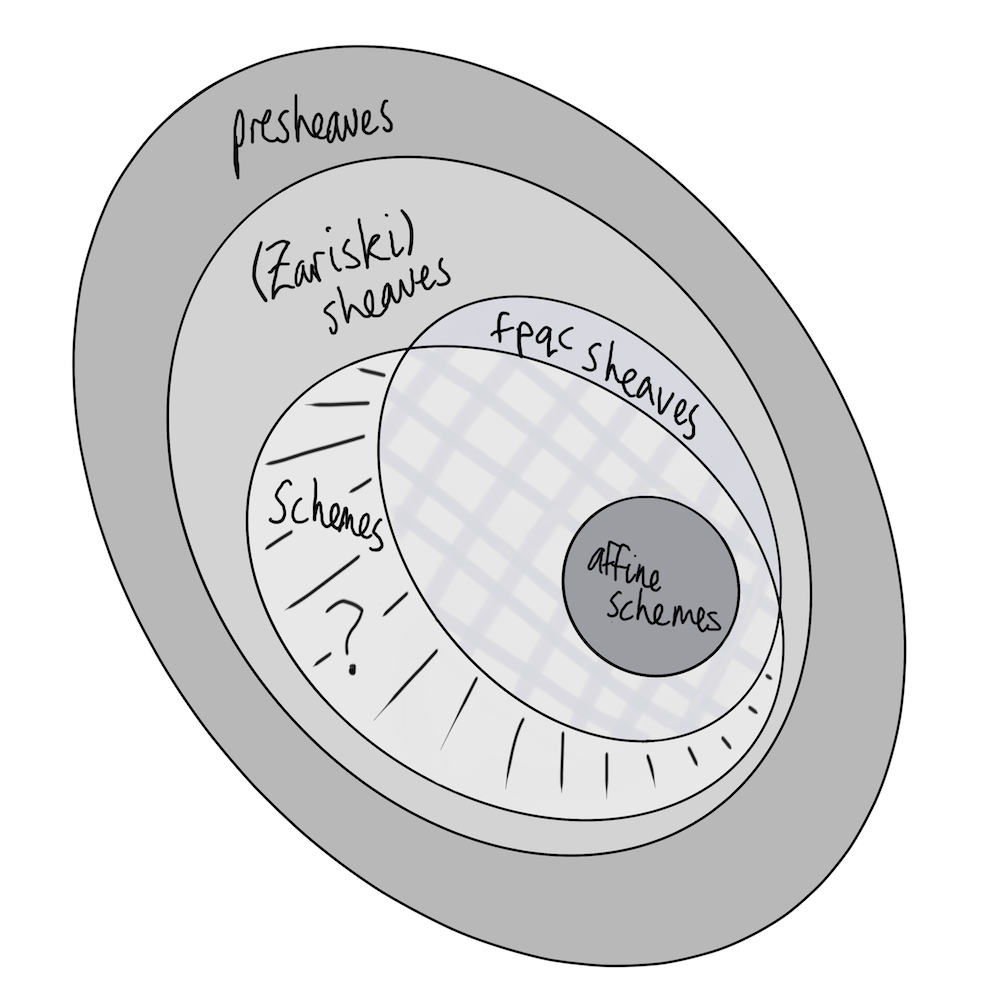
\includegraphics[width=\textwidth]{images/hierarchy.png}}
            \end{minipage}
            \hfill
            \begin{minipage}[t]{0.33\textwidth}
                \vspace{0pt}
                \caption{The hierarchy, considering objects up to isomorphism -- really there are `lots more' fpqc sheaves than schemes: $\Shv^{\text{fpqc}}(\aff{\ccat})$ is bicomplete but $\Sch(\ccat)$ does \emph{not} have all colimits, so we can construct $X\in\Shv^{\text{fpqc}}(\aff{\ccat})\setminus\Sch(\ccat)$ by talking a sufficiently nasty colimit\\\textbf{Note:} it seems possible (hence the question mark) that $\Sch(\ccat)\subset\Shv^\text{fpqc}(\aff{\ccat})$, since Zariski open morphisms are also flat morphisms, and we have an `fpqc-sheafification' functor $\Shv(\aff{\ccat})\to\Shv^\text{fpqc}(\aff{\ccat})$ that is a left adjoint (and so preserves colimits) -- this is not mentioned in \cite{Toen:2005wxa} and we don't have the space here to go any further}\label{fg:hierarchy}
            \end{minipage}
        \end{figure}

        % \begin{equation*}\label{eq:full-diagram-of-inclusions}
        %     \begin{array}{ccccccccccc}
        %         & &\tightoverset{fpqc sheaves}{\big\downarrow} & & & &\tightoverset{schemes}{\big\downarrow} & & & &\tightoverset{presheaves}{\big\downarrow}\\
        %         \aff{\ccat} &\twoheadrightarrow &\Shv^{\text{fpqc}}(\aff{\ccat}) &\subset &\ASch(\ccat) &\subset &\Sch(\ccat) &\subset&\Shv(\aff{\ccat}) &\subset &\PShv(\aff{\ccat}).\\
        %         \tightunderset{affine schemes}{\big\uparrow} & & & &\tightunderset{affine schemes}{\big\uparrow} & & & &\tightunderset{(Zariski) sheaves}{\big\uparrow} & &
        %     \end{array}
        % \end{equation*}
        


    % subsubsection partial_summary (end)



    \subsubsection{Properties of schemes} % (fold)
    \label{ssub:properties_of_schemes}

        We now state some fundamental properties of schemes, and refer the reader to \cite{Toen:2005wxa} for proofs of each one.
        However, there are diagrams (at the end of this section) of sketches for most of the proofs, which should hopefully convey the main ideas reasonably well.
        The conventions used in these diagrams is explained in \cref{fg:diagram-key}.
        We recall that we can think of pullbacks as a generalisation of fibres; that pullbacks of epimorphisms are epimorphisms; and that pullbacks of Zariski open morphisms are Zariski open.
        
        % \begin{figure}[h]
        %     \floatbox[{\capbeside\thisfloatsetup{capbesideposition={right,top},capbesidewidth=4.5cm}}]{figure}[\FBwidth]
        %     {\caption{The diagram corresponding to the statement `if a sheaf $F$ has an affine Zariski cover $\{A_i\}$ then it is a scheme' -- the lighter grey corresponds to the hypotheses on $F$ -- note that we don't have any notation for whether or not a map is Zariski open, in an attempt to retain simplicity}\label{fg:example-diagram}}
        %     {\frame{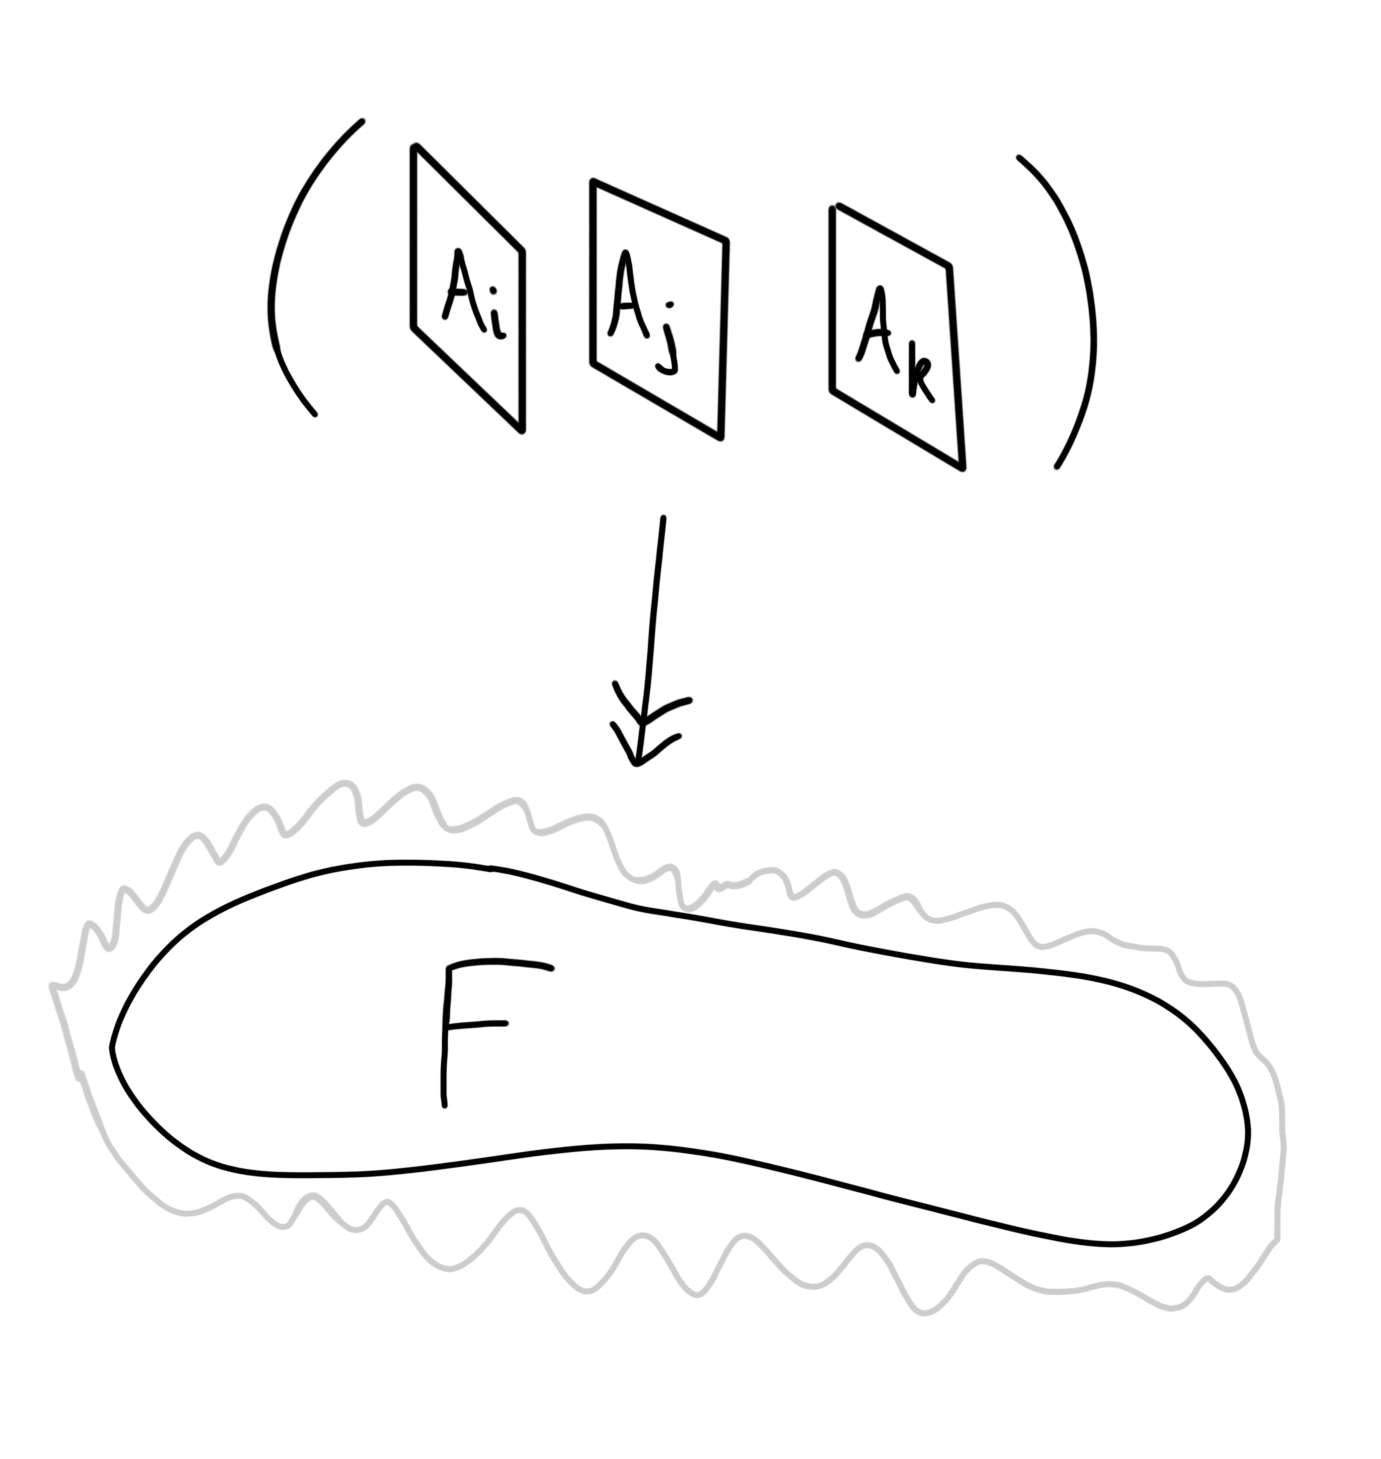
\includegraphics[width=.4\textwidth]{images/example-diagram.png}}}
        % \end{figure}

        % A fundamental property of relative schemes is that of \emph{recollement}.

        \begin{lemma}[Gluing and affine schemes {(Proposition~2.6,~\S2.4,~p.20)}]\label{le:recollement-and-affine}
            \mbox{}\vspace{-1em}
            \begin{enumerate}[(i)]
                \item Let $A,B$ be affine schemes, $G$ a sheaf, and $G\to A\leftarrow B$ morphisms of sheaves.
                    If $G$ is a scheme then $F=B\times_A G$ is also a scheme.
                \item Let $A$ be an affine scheme, $F$ a sheaf, and $F\to A$ a morphism of sheaves.
                    If there exists an affine Zariski cover $\{A_i\to A\}$ such that each $F\times_A A_i$ is a scheme then $F$ is a scheme.\qedhere
            \end{enumerate}
        \end{lemma}

        % \begin{proof}
        %     See \cite{Toen:2005wxa}.
        % \end{proof}

        % We now note a few more useful properties of schemes that follow from what we have so far, pausing along the way only to make another category theoretical definition.







        \clearpage






        \begin{lemma}[\mbox{}{Proposition~2.17,~\S2.4,~p.21}]
            \mbox{}\vspace{-1em}
            \begin{enumerate}[(i)]
                \item Let $F$ be a scheme and $F_0\subset F$ be Zariski open in the sense of \cref{df:zariski-open-sheaves}.
                    Then $F_0$ is a scheme.
                \item Let $f\colon F\to G$ be a morphism between schemes.
                    Then $f$ is Zariski open in the sense of \cref{df:zariski-open-sheaves} if and only if $f$ satisfies the following two conditions:
                    \begin{enumerate}
                        \item $f$ is a monomorphism;
                        \item there exists an affine Zariski cover $\{X_i\to F\}$ such that each morphism $X_i\to G$ given by composition with $f$ is Zariski open.\qedhere
                    \end{enumerate}
            \end{enumerate}
        \end{lemma}

        % \begin{proof}
        %     See \cite{Toen:2005wxa}.
        % \end{proof}

        % Before the next lemma, which lets us think of a scheme as being glued together from affine schemes, we give a rough definition of a \emph{congruence on an object}, and refer the reader to \cite{Anonymous:_jtXUz4d} for precise details.

        \begin{definition}[Congruence on an object]
            For $X\in\dcat$, a congruence $R$ on $X$ is\footnote{
                Up to some notion of isomorphism between morphisms -- see \cite{Anonymous:_jtXUz4d}.
            } a monomorphism
            \begin{equation*}
                R\overset{(p_1,p_2)}{\hookrightarrow} X\times X
            \end{equation*}
            equipped with the following morphisms:
            \begin{enumerate}[(i)]
                \item (\emph{reflexivity}) $r\colon X\to R$ such that $p_1\circ r=p_2\circ r=\id_X$;
                \item (\emph{symmetry}) $s\colon R\to R$ such that $p_1\circ s=p_2$ and $p_2\circ s=p_1$;
                \item (\emph{transitivity}) $t\colon R\times_X R\to R$ such that
                    \begin{equation*}
                        \begin{tikzcd}[column sep=2em, row sep=2.5em]
                            R\times_X R \arrow[r, swap, "\pi_1"] \arrow[r, bend left=50, "t"] \arrow[d, "\pi_2"] \arrow[d, bend right=50, swap, "t"] & R \arrow[d, "p_1"]\\
                            R \arrow[r, swap, "p_2"] & X
                        \end{tikzcd}
                    \end{equation*}
                    commutes (where $\pi_1$, $\pi_2$ are the pullback morphisms).
            \end{enumerate}
            Given such an $R$, we define the \emph{quotient object $X/R$} as
            \begin{equation*}
                X/R=\coeq(R\overset{p_1}{\underset{p_2}{\rightrightarrows}} X).\qedhere
            \end{equation*}
        \end{definition}


        \begin{lemma}[Stability; gluing affine schemes {(Proposition~2.18,~\S2.4,~p.21)}]\label{le:actual-gluing}
            \mbox{}\vspace{-1em}
            \begin{enumerate}[(i)]
                \item The subcategory $\Sch(\ccat)\subset\Shv(\aff{\ccat})$ is stable under disjoint unions and pullbacks.
                \item A sheaf $F\in\Shv(\aff{\ccat})$ is a scheme if and only if there exists some congruence $R$ on some sheaf $X\in\Shv(\aff{\ccat})$ where the following four conditions are satisfied:
                \begin{enumerate}
                    \item $X\cong\coprod_{i\in I}U_i$ for some affine schemes $U_i$;
                    \item for all $(i,j)\in I^2$, the subsheaf $R_{i,j}\subset U_i\times U_j$ given by the pullback\footnote{
                        `Intersecting down' the congruence: $R\cong\coprod_{i,j}R_{i,j}$.
                        The morphisms $U_i\times U_j\to X\times X$ are those induced by the $U_i\to\coprod U_i\congto X$.
                    }
                        \begin{equation*}
                            \begin{tikzcd}[column sep=1em]
                                R_{i,j} \arrow[r] \arrow[d] & U_i\times U_j \arrow[d]\\
                                R \arrow[r] & X\times X
                            \end{tikzcd}
                        \end{equation*}
                        is such that each induced morphism
                        \begin{equation*}
                            R_{i,j}\to U_i
                        \end{equation*}
                        is Zariski open;
                    \item for each $i\in I$ the subobject $R_{i,i}\subset U_i\times U_i$ is equal to the image of the diagonal morphism $U_i\to U_i\times U_i$;
                    \item $F\cong X/R$.\qedhere
                \end{enumerate}
            \end{enumerate}
        \end{lemma}

        % \begin{proof}
        %     See \cite{Toen:2005wxa}.
        % \end{proof}

        % The reason that this lemma is so important is because it confirms our hope that schemes are `affine schemes glued together in a nice way'.
        % Part (i) says that if we place two schemes side-by-side (i.e. trivially glue them) or `intersect' (\textbf{TJH again, is `intersect' the right word here?}) them, then the result is also a scheme.
        % Part (ii) says that a scheme is exactly what we get if we take some affine schemes $U_i$ with affine subschemes $V_i\subset U_i$ such that the inclusion is Zariksi open, and identify some $V_j$ with $V_i$ in a suitably nice way.
        It is possible to rephrase \cref{le:actual-gluing}(ii) in terms of pushouts.
        Say we have affine schemes $A,X,Y$ and Zariski-open immersions $A\to X$, $A\to Y$.
        Then $X\coprod_A Y$ is the presheaf obtained by gluing $X$ and $Y$ along the images of $A$ (see \cref{fg:gluing}).
        The above lemma then says that this presheaf is also actually a scheme.

        % \begin{figure}[h!]
        %     \centering
        %     \frame{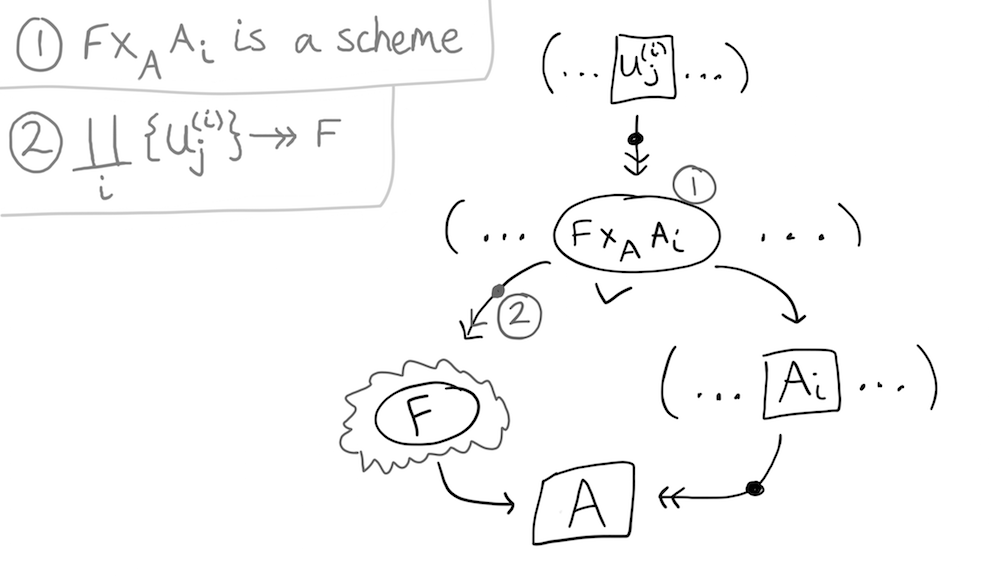
\includegraphics[width=\textwidth]{images/recollement-affine-ii-new.png}}
        %     \caption{\cref{le:recollement-and-affine}(ii) -- \emph{this lemma is a special case of \cite[Lemme~2.20,~\S2.4]{Toen:2005wxa}} -- for \numberincircle{1} the previous part of the lemma tells us that \mbox{$F\times_A A_i$} is a scheme; \numberincircle{2} says that if we take affine covers for all of the \mbox{$F\times_A A_i$} then together they cover $F$}\label{fg:recollement-affine-ii}
        % \end{figure}

        % \begin{figure}[h!]
        %     \centering
        %     \begin{minipage}[t]{0.4\textwidth}
        %         \vspace{0pt}
        %         \frame{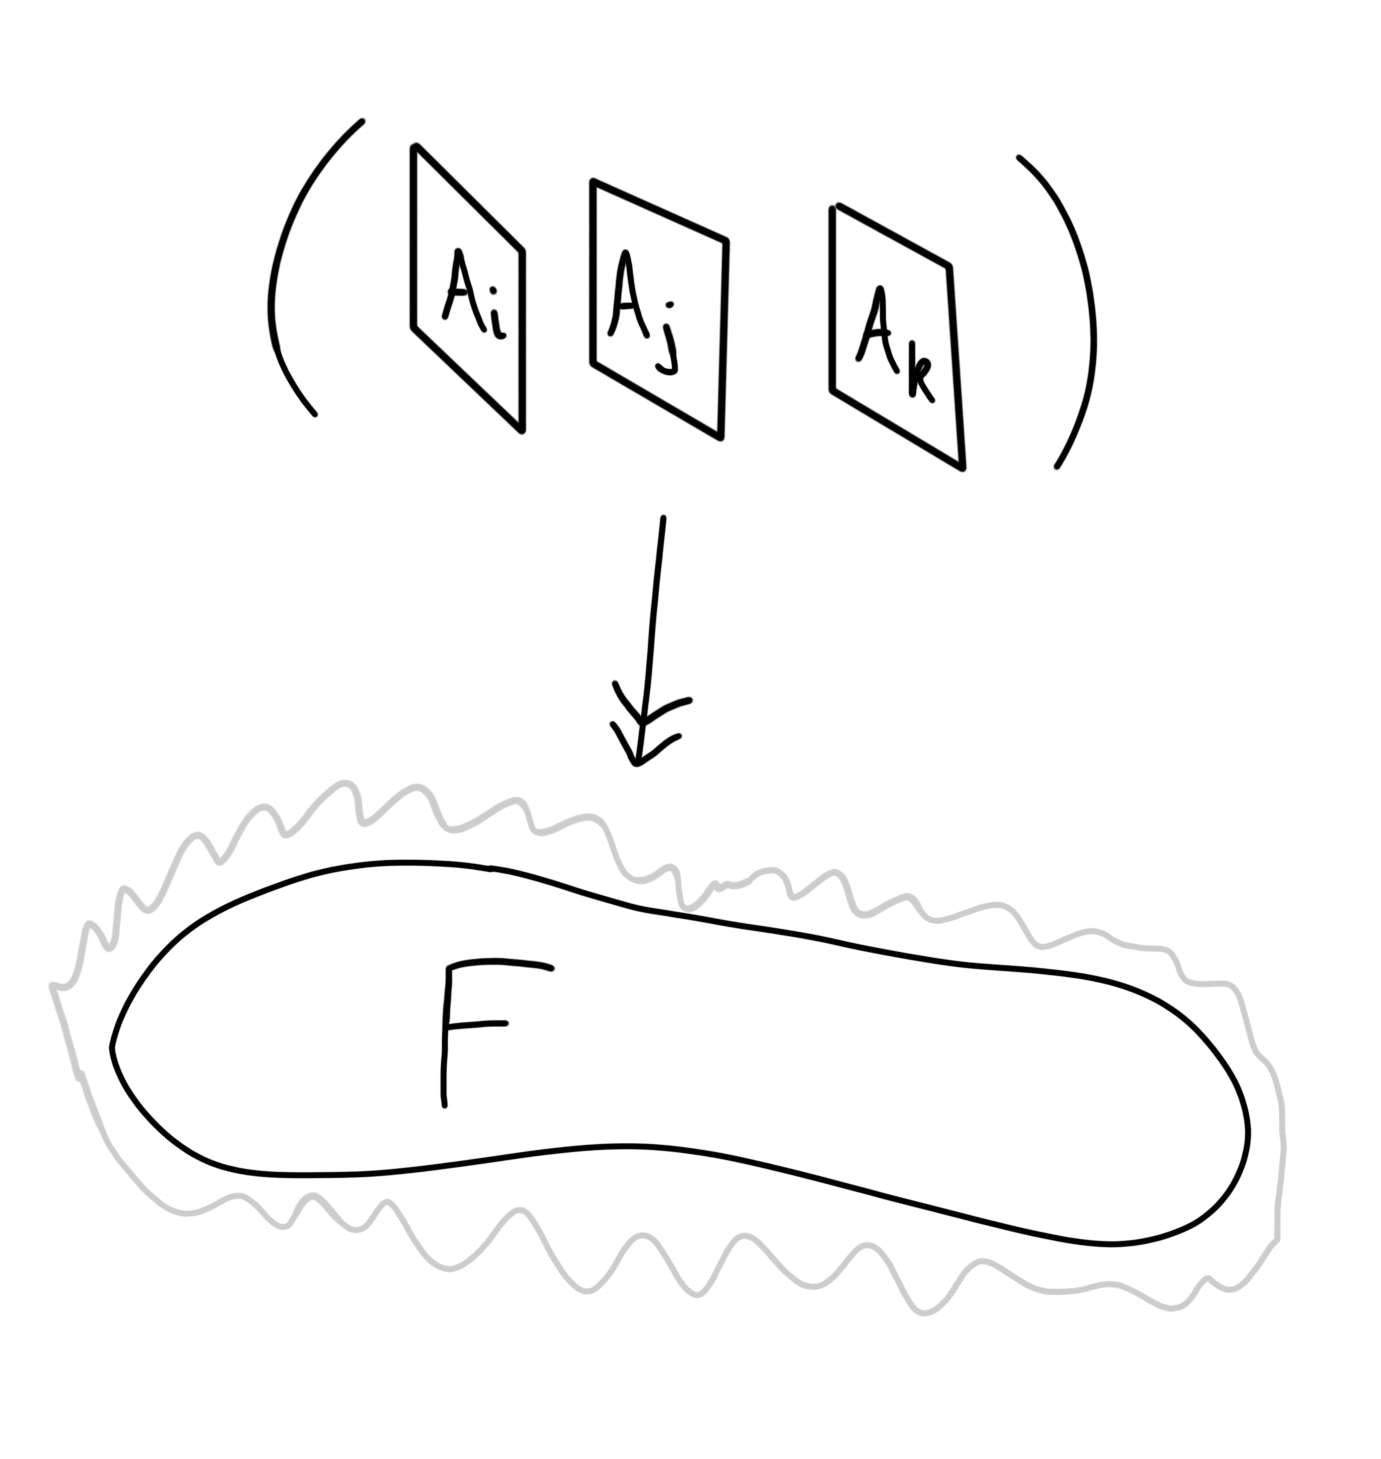
\includegraphics[width=\textwidth]{images/example-diagram.png}}
        %     \end{minipage}
        %     \hspace{0.02\textwidth}
        %     \begin{minipage}[t]{0.48\textwidth}
        %         \vspace{0pt}
        %         \caption{The diagram corresponding to the statement `if a sheaf $F$ has an affine Zariski cover $\{A_i\}$ then it is a scheme' -- the lighter grey corresponds to the hypotheses on $F$ -- in an attempt to retain simplicity here we don't use any notation to show if a map is Zariski open}\label{fg:example-diagram}
        %     \end{minipage}
        % \end{figure}

        % \begin{figure}[p]
        %     \centering
        %     \begin{minipage}[t]{0.73\textwidth}
        %         \vspace{0pt}
        %         \frame{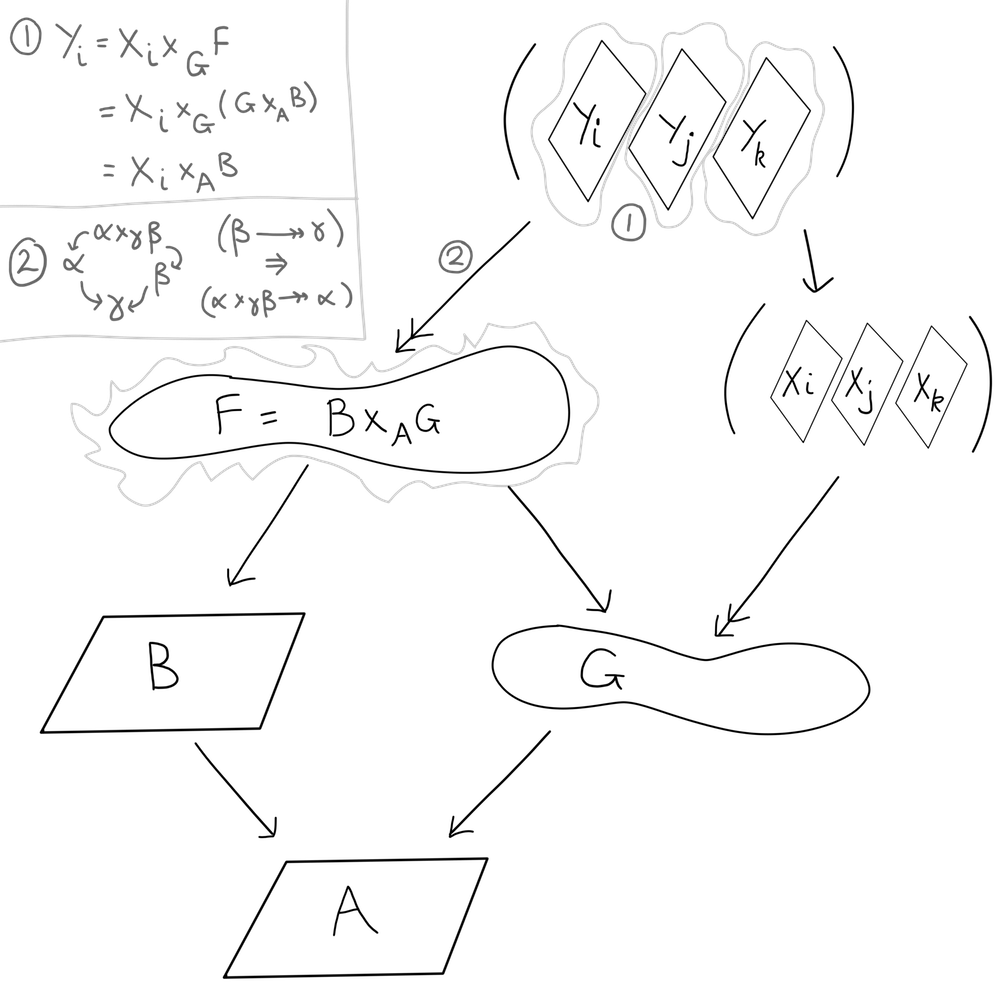
\includegraphics[width=\textwidth]{images/recollement-affine-i.png}}
        %         \caption{\Cref{le:recollement-and-affine}(i)}\label{fg:recollement-affine-i}
        %     \end{minipage}
        %     \hfill
        %     \begin{minipage}[t]{0.23\textwidth}
        %         \vspace{0pt}
        %         {\footnotesize The proof of \numberincircle{1} uses \emph{pasting of pullbacks} and tells us that the $Y_i$ are affine schemes, because \mbox{$\spec\alpha\times_{\spec\beta}\spec\gamma$} \mbox{$\cong\spec(\alpha\coprod_\beta\gamma)$};}
        %         % \begin{align*}
        %         %     &\spec\alpha\times_{\spec\beta}\spec\gamma\\
        %         %     &\cong\spec(\alpha\coprod_\beta\gamma);
        %         % \end{align*}
        %         {\footnotesize the proof of \numberincircle{2} simply says that the pullback of an epimorphism is also an epimorphism}
        %     \end{minipage}
        % \end{figure}

        % \begin{figure}[p]
        %     \centering
        %     \begin{minipage}[t]{0.73\textwidth}
        %         \vspace{0pt}
        %         \frame{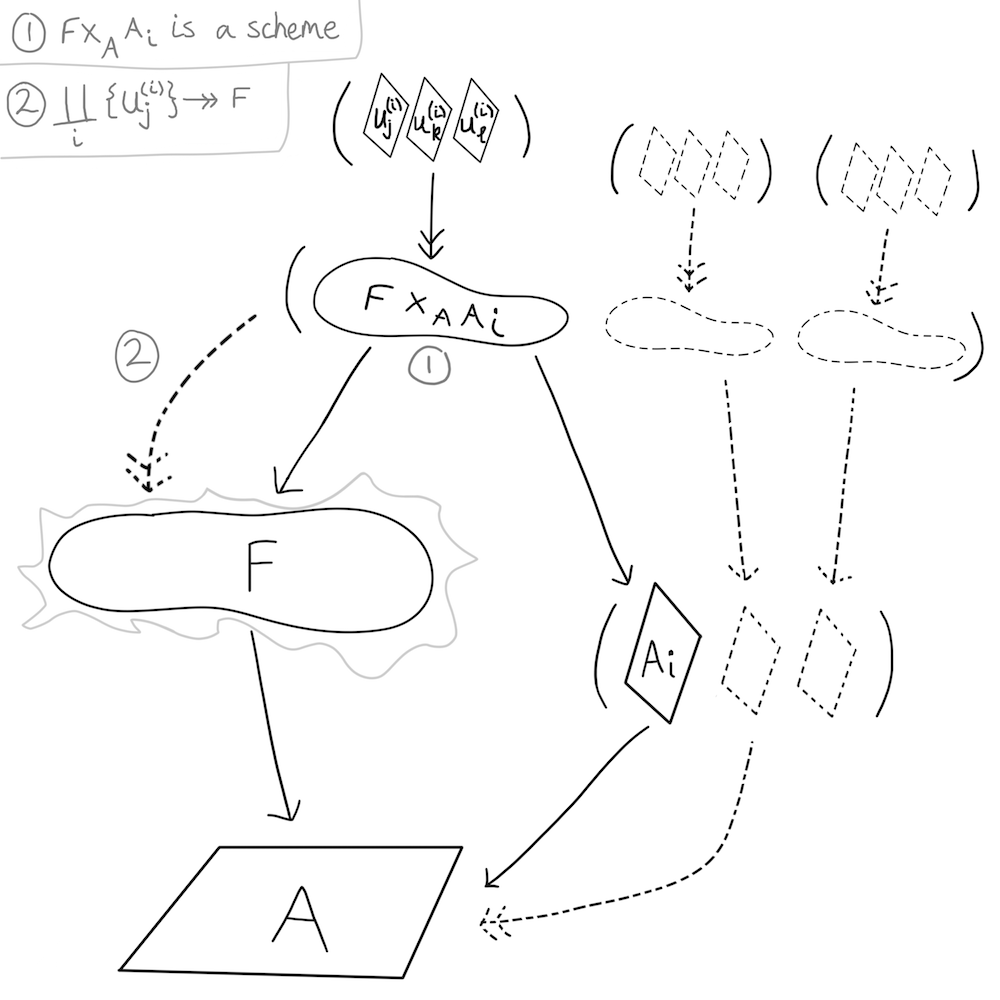
\includegraphics[width=\textwidth]{images/recollement-affine-ii.png}}
        %         \caption{\Cref{le:recollement-and-affine}(ii)}\label{fg:recollement-affine-ii}
        %     \end{minipage}
        %     \hfill
        %     \begin{minipage}[t]{0.23\textwidth}
        %         \vspace{0pt}
        %         {\footnotesize For \numberincircle{1} the previous part of the lemma tells us that \mbox{$F\times_A A_i$} is a scheme; \numberincircle{2} says that if we take affine covers for all of the \mbox{$F\times_A A_i$} then together they cover~$F$}
        %     \end{minipage}
        % \end{figure}

        \begin{figure}[h!]
            \centering
            \frame{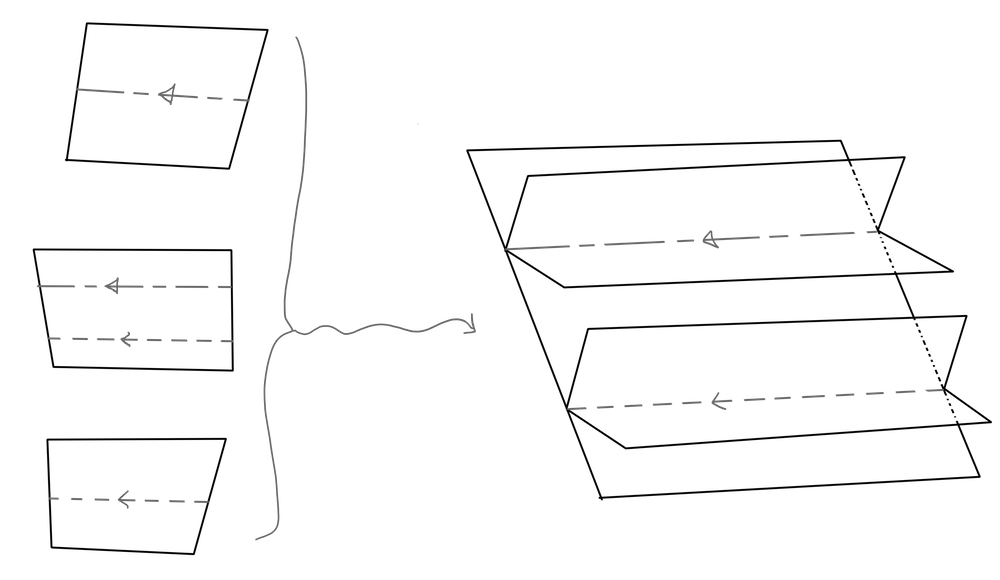
\includegraphics[width=.6\textwidth]{images/gluing.png}}
            \caption{Rephrasing \cref{le:actual-gluing}(ii) in familiar `gluing' terms -- if we take some affine schemes with Zariski-open affine subschemes and glue along these subschemes in a `sufficiently nice' way, then we end up with a scheme -- further, every scheme is obtained in exactly this way -- \emph{schemes are affine schemes glued together}}\label{fg:gluing}
        \end{figure}

    % subsubsection properties_of_schemes (end)





    \subsubsection{Another view} % (fold)
    \label{ssub:another_view}

        Here we briefly discuss how the functor of points approach that we have been using (\cref{sub:background_knowledge}) coincides with the classical ringed space approach.
        % As mentioned in \cref{sub:background_knowledge}, we have been using the functor of points approach, but we now discuss how we could have instead used the ringed space approach, and how these two notions coincide.
        What follows is a sketch of the story -- in particular we make claims without stating proofs -- and we refer the reader to the end (the last four paragraphs) of \cite[\S2.4, p.24]{Toen:2005wxa} as well as \cite[\S IX.1--3]{MacLane:1992uz} for the details.

        \bigskip

        Given some topological space $T$ we can view the category $\Op{T}$ as a lattice, with partial order given by inclusion.
        Generally, define a \emph{frame} to be any lattice $X$ that behaves suitably like $\Op{T}$: having arbitrary joins and finite meets, and meets distributing over arbitrary joins.
        The morphisms between frames are maps of partially-ordered sets preserving arbitrary joins and finite meets.
        This defines a category $\Fra$ of frames.
        We define the category of \emph{locales}\footnote{
            Translation note: locales are called \emph{lieux} in French.
        } as $\Loc=\op{\Fra}$, and for $f\colon X\to Y$ in $\Loc$ we write $f^{-1}\colon\mathcal{O}(Y)\to\mathcal{O}(X)$ to be the corresponding morphism of objects in $\Fra$.

        Next, given a locale $X$ we can define \emph{points of $X$} as locale morphisms $1\to X$, where $1\in\Loc$ is the terminal locale.
        We say that a locale \emph{has enough points} if elements of the lattice can be distinguished by a single point\footnote{
            \Cite[\S IX.2]{MacLane:1992uz} provides a nice way of thinking of this in terms of frames.
        }.
        That is, for any distinct $U,V\in\mathcal{O}(X)$, there exists $p\colon\singleton\to X$ such that $p^{-1}(U)\neq p^{-1}(V)$.
        It can be shown\footnote{
            \cite[Corollary~4,~\S IX.3]{MacLane:1992uz}
        } that if a locale $X$ has enough points then there exists some topological space $|X|$ such that $\mathcal{O}(X)\cong\Op{|X|}$.

        Finally, given $X\in\Sch(\ccat)$, we define $\Zar{X}$ as the full subcategory of $\Shv(\aff{\ccat})/X$ consisting of $u\colon Y\to X$ such that $Y$ is a scheme and $u$ is an open Zariski immersion.
        It turns out that $\Zar{X}$ is a locale, and it has an induced topology coming from the canonical topology on $\Shv(\aff{\ccat})$.
        If we define $\AffZar{X}$ to be the full subcategory of $\Zar{X}$ consisting of $Y\to X$ with $Y$ an affine scheme, and endow this with the same restricted topology, then we have the equivalence of categories
        \begin{equation*}
            \Shv(\Zar{X})\equiv\Shv(\AffZar{X}),
        \end{equation*}
        so we write $\Shv(X_\text{Zar})$ to mean either (under this identification).
        The topology on $\Zar{X}$ is generated by a quasi-compact pretopology (i.e. finite covering families), namely $\AffZar{X}$.
        This means that $\Zar{X}$ has enough points\footnote{
            More generally, \emph{Deligne's theorem} (\cite[Corollary~3,~\S IX.11]{MacLane:1992uz}) tells us that any \emph{coherent topos} has enough points.
        }, and so, by the above, $\Zar{X}\equiv\Op{|X|}$ for some topological space $|X|$.
        This induces the equivalence
        \begin{equation*}
            \Shv(X_\text{Zar})\equiv\Shv(|X|).
        \end{equation*}

        \bigskip

        Now let $Y=(\spec A\to X)\in\AffZar{X}$.
        We can associate to $Y$ the object $A\in\comm{\ccat}$; letting $Y$ vary over $\AffZar{X}$ induces a functor
        \begin{align*}
            \mathcal{O}_X\colon\op{\AffZar{X}}&\to\comm{\ccat}\\
            (X\to\spec A)&\mapsto A.
        \end{align*}
        Then $\mathcal{O}_X$ is a sheaf\footnote{
            \Cref{le:essential-image-is-fpqc}
        }, and the pair $(|X|,\mathcal{O}_X)$ acts as in a $\ccat$-ringed space approach.
        Replacing $\ccat$ with $\Ab$ we recover the classical ringed space approach.

    % subsubsection another_view (end)


        \begin{figure}[h!]
            \centering
            \frame{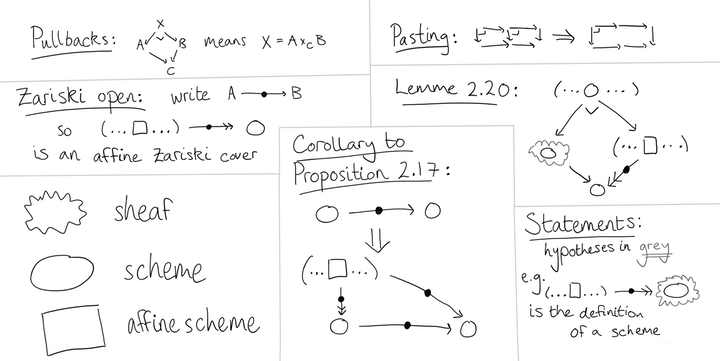
\includegraphics[width=\textwidth]{images/diagram-key-new.png}}
            \caption{The motivation of the notation is the naive motto `straight lines are simpler than curved ones': affine schemes are our building blocks, schemes are slightly more complicated, and sheaves are the least well behaved of all -- \emph{the choice of graphical notation is not meant to be read into too deeply}}
            \label{fg:diagram-key}
        \end{figure}

        \begin{figure}[h!]
            \centering
            \frame{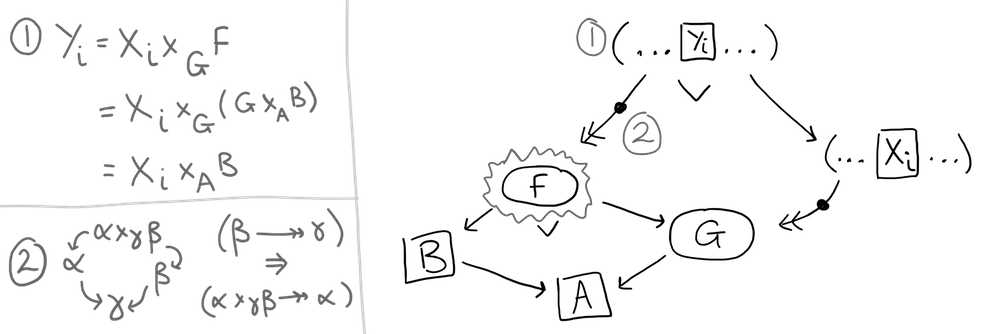
\includegraphics[width=\textwidth]{images/recollement-affine-i-new.png}}
            \caption{\cref{le:recollement-and-affine}(i) -- the proof of \numberincircle{1} uses \emph{pasting of pullbacks} and tells us that the $Y_i$ are affine schemes, because $\spec\alpha\times_{\spec\beta}\spec\gamma\cong\spec(\alpha\coprod_\beta\gamma)$; the proof of \numberincircle{2} simply says that the pullback of an epimorphism is also an epimorphism}\label{fg:recollement-affine-i}
        \end{figure}


        \begin{figure}[h!]
            \centering
            \begin{minipage}[t]{0.73\textwidth}
                \vspace{0pt}
                \frame{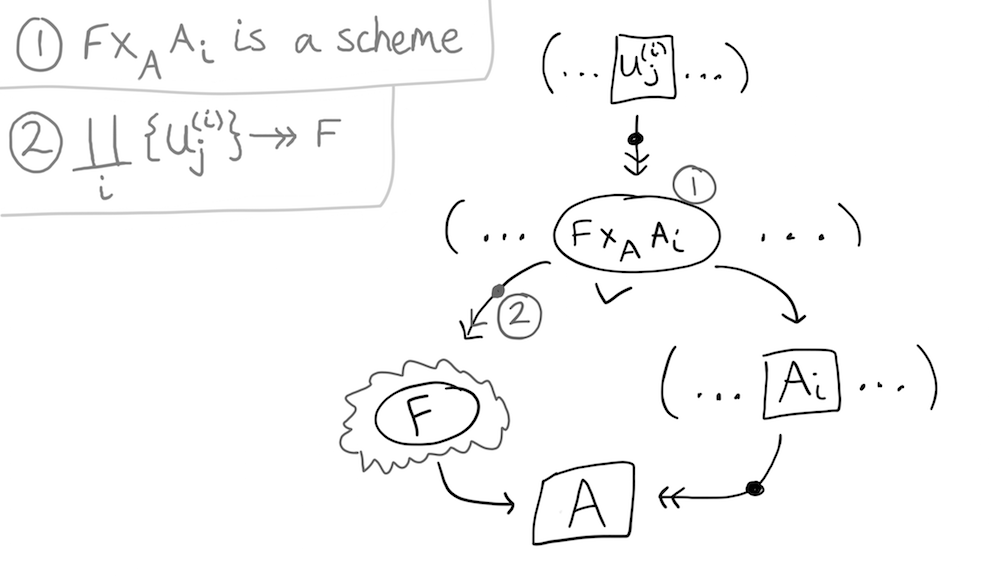
\includegraphics[width=\textwidth]{images/recollement-affine-ii-new.png}}
                \caption{\Cref{le:recollement-and-affine}(ii) -- a special case of \cite[Lemme~2.20,~\S2.4]{Toen:2005wxa}}\label{fg:recollement-affine-ii}
            \end{minipage}
            \hfill
            \begin{minipage}[t]{0.23\textwidth}
                \vspace{0pt}
                {\footnotesize For \numberincircle{1} the previous part of the lemma tells us that \mbox{$F\times_A A_i$} is a scheme; \numberincircle{2} says that if we take affine covers for all of the \mbox{$F\times_A A_i$} then together they cover~$F$}
            \end{minipage}
        \end{figure}

        \begin{figure}[h!]
            \centering
            \begin{minipage}[t]{0.73\textwidth}
                \vspace{0pt}
                \frame{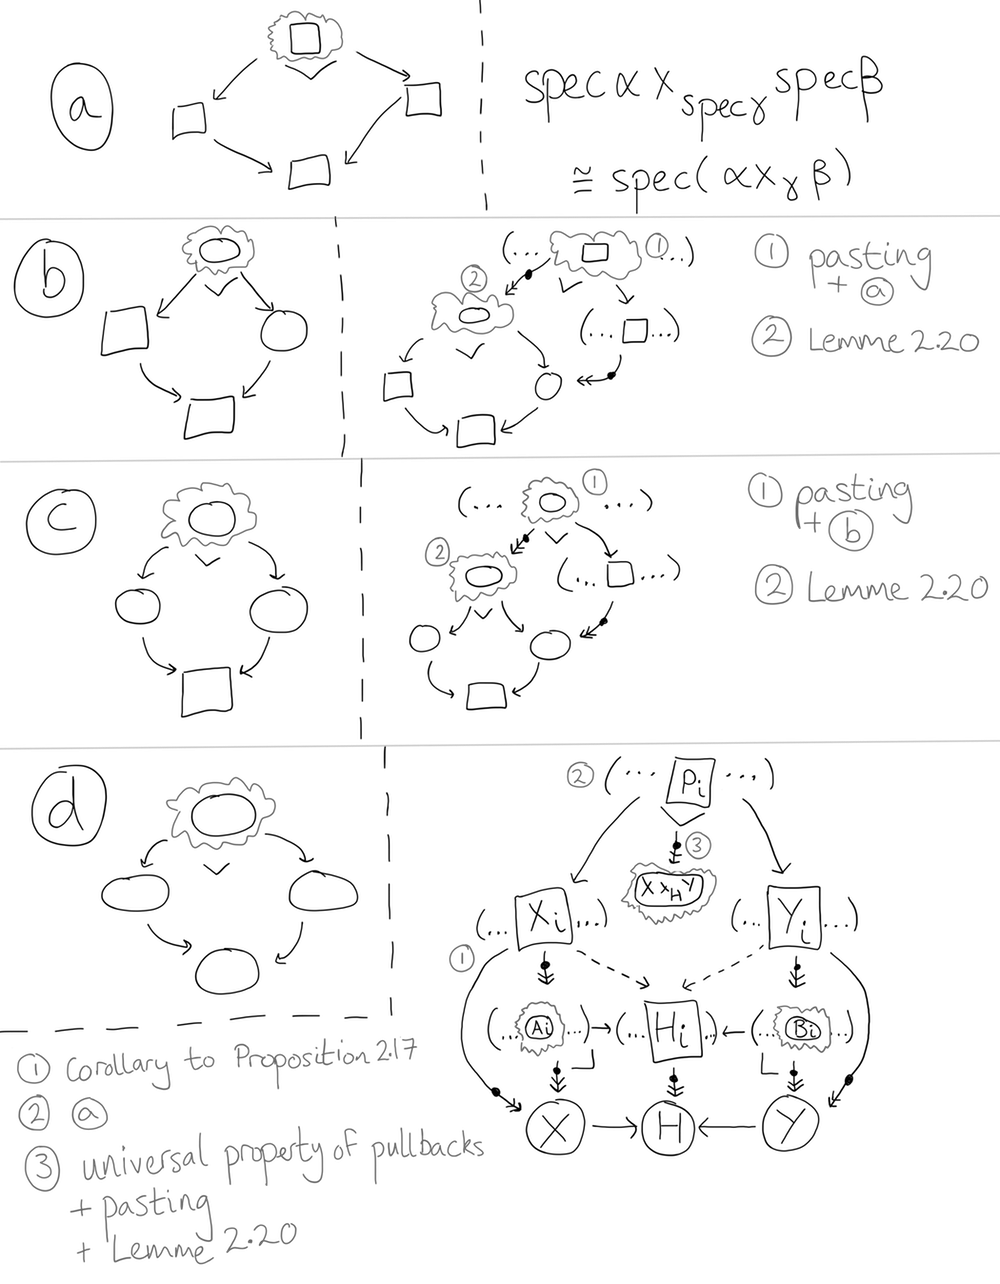
\includegraphics[width=\textwidth]{images/stability.png}}
                \caption{\Cref{le:actual-gluing}(i) -- the statement concerning pullbacks}\label{fg:stability}
            \end{minipage}
            \hfill
            \begin{minipage}[t]{0.23\textwidth}
                \vspace{0pt}
                {\footnotesize We build up to this proof in successive steps, from \numberincircle{a} to \numberincircle{d} -- the statements are on the left and the proofs on the right}
            \end{minipage}
        \end{figure}



% subsection schemes (end)
